\documentclass{standalone}
\usepackage{tikz}
\usepackage{ctex,siunitx}
\setCJKmainfont{Noto Serif CJK SC}
\usepackage{tkz-euclide}
\usepackage{amsmath}
\usetikzlibrary{patterns, calc}
\usetikzlibrary {decorations.pathmorphing, decorations.pathreplacing, decorations.shapes,}
\begin{document}
\small
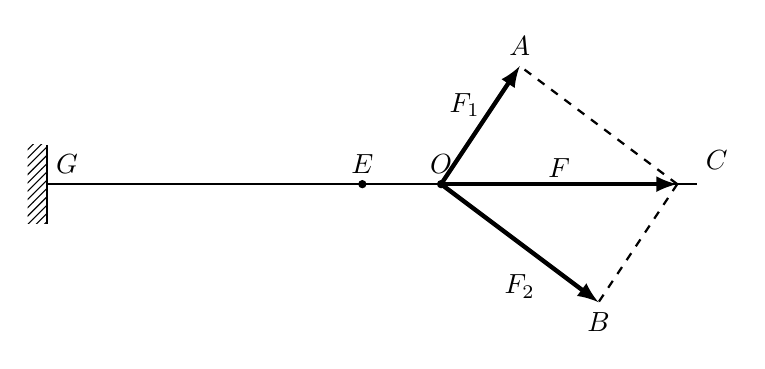
\begin{tikzpicture}[>=latex, thick,scale=1]
  % \useasboundingbox(-1,-0.75)rectangle(3.7,1.4);
  \fill [pattern = north east lines] (0.75+1,0) rectangle (1+1,1);
  \draw (1+1,1)--(1+1,0);
  \draw (2,0.5)--(10.25,0.5);
  \node at (1.25+1, 0.75){$G$};
  \fill (6, .5) circle[radius=1.5pt];
  \fill (7, .5) circle[radius=1.5pt];
  \node at (6, 0.75){$E$};
  \node at (7, 0.75){$O$};
  \draw [->, ultra thick](7, .5)--(8,2);
  \draw [->, ultra thick](7, .5)--(9,-1);
  \draw [dashed](10, .5)--(8,2);
  \draw [dashed](10, .5)--(9,-1);
  \node at (8.5, .7){$F$};
  \node at (10.5, 0.8){$C$};
  \node at (8,2.25){$A$};
  \node at (9,-1.25){$B$};
  \draw [->, ultra thick](7, .5)--(10,.5);
  \node at (7.3, 1.5){$F_1$};
  \node at (8, -0.8){$F_2$};
\end{tikzpicture}
\end{document}